\documentclass[
  man,
  floatsintext,
  longtable,
  nolmodern,
  notxfonts,
  notimes,
  colorlinks=true,linkcolor=blue,citecolor=blue,urlcolor=blue]{apa7}

\usepackage{amsmath}
\usepackage{amssymb}



\usepackage[bidi=default]{babel}
\babelprovide[main,import]{british}


% get rid of language-specific shorthands (see #6817):
\let\LanguageShortHands\languageshorthands
\def\languageshorthands#1{}

\RequirePackage{longtable}
\RequirePackage{threeparttablex}

\makeatletter
\renewcommand{\paragraph}{\@startsection{paragraph}{4}{\parindent}%
	{0\baselineskip \@plus 0.2ex \@minus 0.2ex}%
	{-.5em}%
	{\normalfont\normalsize\bfseries\typesectitle}}

\renewcommand{\subparagraph}[1]{\@startsection{subparagraph}{5}{0.5em}%
	{0\baselineskip \@plus 0.2ex \@minus 0.2ex}%
	{-\z@\relax}%
	{\normalfont\normalsize\bfseries\itshape\hspace{\parindent}{#1}\textit{\addperi}}{\relax}}
\makeatother




\usepackage{longtable, booktabs, multirow, multicol, colortbl, hhline, caption, array, float, xpatch}
\usepackage{subcaption}


\renewcommand\thesubfigure{\Alph{subfigure}}
\setcounter{topnumber}{2}
\setcounter{bottomnumber}{2}
\setcounter{totalnumber}{4}
\renewcommand{\topfraction}{0.85}
\renewcommand{\bottomfraction}{0.85}
\renewcommand{\textfraction}{0.15}
\renewcommand{\floatpagefraction}{0.7}

\usepackage{tcolorbox}
\tcbuselibrary{listings,theorems, breakable, skins}
\usepackage{fontawesome5}

\definecolor{quarto-callout-color}{HTML}{909090}
\definecolor{quarto-callout-note-color}{HTML}{0758E5}
\definecolor{quarto-callout-important-color}{HTML}{CC1914}
\definecolor{quarto-callout-warning-color}{HTML}{EB9113}
\definecolor{quarto-callout-tip-color}{HTML}{00A047}
\definecolor{quarto-callout-caution-color}{HTML}{FC5300}
\definecolor{quarto-callout-color-frame}{HTML}{ACACAC}
\definecolor{quarto-callout-note-color-frame}{HTML}{4582EC}
\definecolor{quarto-callout-important-color-frame}{HTML}{D9534F}
\definecolor{quarto-callout-warning-color-frame}{HTML}{F0AD4E}
\definecolor{quarto-callout-tip-color-frame}{HTML}{02B875}
\definecolor{quarto-callout-caution-color-frame}{HTML}{FD7E14}

%\newlength\Oldarrayrulewidth
%\newlength\Oldtabcolsep


\usepackage{hyperref}




\providecommand{\tightlist}{%
  \setlength{\itemsep}{0pt}\setlength{\parskip}{0pt}}
\usepackage{longtable,booktabs,array}
\usepackage{calc} % for calculating minipage widths
% Correct order of tables after \paragraph or \subparagraph
\usepackage{etoolbox}
\makeatletter
\patchcmd\longtable{\par}{\if@noskipsec\mbox{}\fi\par}{}{}
\makeatother
% Allow footnotes in longtable head/foot
\IfFileExists{footnotehyper.sty}{\usepackage{footnotehyper}}{\usepackage{footnote}}
\makesavenoteenv{longtable}

\usepackage{graphicx}
\makeatletter
\newsavebox\pandoc@box
\newcommand*\pandocbounded[1]{% scales image to fit in text height/width
  \sbox\pandoc@box{#1}%
  \Gscale@div\@tempa{\textheight}{\dimexpr\ht\pandoc@box+\dp\pandoc@box\relax}%
  \Gscale@div\@tempb{\linewidth}{\wd\pandoc@box}%
  \ifdim\@tempb\p@<\@tempa\p@\let\@tempa\@tempb\fi% select the smaller of both
  \ifdim\@tempa\p@<\p@\scalebox{\@tempa}{\usebox\pandoc@box}%
  \else\usebox{\pandoc@box}%
  \fi%
}
% Set default figure placement to htbp
\def\fps@figure{htbp}
\makeatother


% definitions for citeproc citations
\NewDocumentCommand\citeproctext{}{}
\NewDocumentCommand\citeproc{mm}{%
  \begingroup\def\citeproctext{#2}\cite{#1}\endgroup}
\makeatletter
 % allow citations to break across lines
 \let\@cite@ofmt\@firstofone
 % avoid brackets around text for \cite:
 \def\@biblabel#1{}
 \def\@cite#1#2{{#1\if@tempswa , #2\fi}}
\makeatother
\newlength{\cslhangindent}
\setlength{\cslhangindent}{1.5em}
\newlength{\csllabelwidth}
\setlength{\csllabelwidth}{3em}
\newenvironment{CSLReferences}[2] % #1 hanging-indent, #2 entry-spacing
 {\begin{list}{}{%
  \setlength{\itemindent}{0pt}
  \setlength{\leftmargin}{0pt}
  \setlength{\parsep}{0pt}
  % turn on hanging indent if param 1 is 1
  \ifodd #1
   \setlength{\leftmargin}{\cslhangindent}
   \setlength{\itemindent}{-1\cslhangindent}
  \fi
  % set entry spacing
  \setlength{\itemsep}{#2\baselineskip}}}
 {\end{list}}
\usepackage{calc}
\newcommand{\CSLBlock}[1]{\hfill\break\parbox[t]{\linewidth}{\strut\ignorespaces#1\strut}}
\newcommand{\CSLLeftMargin}[1]{\parbox[t]{\csllabelwidth}{\strut#1\strut}}
\newcommand{\CSLRightInline}[1]{\parbox[t]{\linewidth - \csllabelwidth}{\strut#1\strut}}
\newcommand{\CSLIndent}[1]{\hspace{\cslhangindent}#1}





\usepackage{newtx}

\defaultfontfeatures{Scale=MatchLowercase}
\defaultfontfeatures[\rmfamily]{Ligatures=TeX,Scale=1}





\title{From Attitudes to Behaviour: The Role of Emotions and Motivation
in Math Choices in Primary School}


\shorttitle{Math Attitudes and Behavioural Choices}


\usepackage{etoolbox}









\authorsnames[{1},{1},{2},{1}]{Riccardo Pagan,Alice Masi,Enrico
Toffalini,Sara Caviola}







\authorsaffiliations{
{Department of Developmental Psychology and Socialization, University of
Padova},{Department of General Psychology, University of Padova}}




\leftheader{Pagan, Masi, Toffalini and Caviola}



\abstract{Math-related behaviours are hard to study in primary school,
where children cannot opt out of mathematics. We used a behavioural task
in which 547 children in Grades 4 and 5 could skip each arithmetic
problem, ask for a hint, or solve it on their own. We initially treated
the three choices as ordered levels of task engagement (skip \textless{}
help \textless{} self), as preregistered. The data offered little
support for this ordinal specification: a multinomial model, which
imposes no order, predicted the choices clearly better than an ordinal
model, and the ordinal model itself required a category-specific effect.
The choices were therefore better described as categories. In the
multinomial model, prior math ability was the strongest predictor. Among
trait attitudes, math avoidance showed the clearest association with
fewer self-reliant responses relative to skipping, although it failed
the CFA screening criterion. State worry was associated specifically
with asking for help. Perceived competence was not a credible predictor,
and academic buoyancy showed an unexpected negative association that
appeared only when the other attitudes were controlled. Behavioural
choices do not seem to lie along a single dimension of engagement;
help-seeking may partly work as masked avoidance. }

\keywords{math anxiety, math avoidance, academic
buoyancy, help-seeking, behavioural measures, multinomial
models, preregistration}

\authornote{\par{\addORCIDlink{Riccardo
Pagan}{0009-0001-5525-8776}}\par{\addORCIDlink{Alice
Masi}{0000-0001-7959-7556}}\par{\addORCIDlink{Enrico
Toffalini}{0000-0002-1404-5133}}\par{\addORCIDlink{Sara
Caviola}{0000-0002-4556-3179}} 
\par{ }
\par{The study design, hypotheses, and analysis plan were preregistered
at \textbf{{[}TODO: OSF link{]}}. Data, code, and materials will be
available at \textbf{{[}TODO: OSF/Zenodo link{]}}.  \textbf{{[}TODO:
conflicts of interest.{]}} \textbf{{[}TODO:
funding.{]}}  \textbf{{[}TODO: CRediT roles.{]}} }
\par{Correspondence concerning this article should be addressed to Sara
Caviola, Department of Developmental Psychology and
Socialization, University of Padova, Via Venezia
8, Padova 35131, Italy, Email: \href{mailto:sara.caviola@unipd.it}{sara.caviola@unipd.it}}
}

\makeatletter
\let\endoldlt\endlongtable
\def\endlongtable{
\hline
\endoldlt
}
\makeatother

\urlstyle{same}



% Single-space table bodies so tables fit in text (floatsintext).
% Wrapped lines inside a cell are set slightly tighter than normal and
% each row gets a little extra vertical air, so a line break inside a
% cell is not mistaken for the start of a new table row.
\usepackage{etoolbox}
\usepackage{array}
% apaquarto writes tables as \begin{table} with no position, i.e. the
% LaTeX default [tbp]: tall tables are then deferred to the end.
\floatplacement{table}{!htbp}
% apaquarto puts each longtable inside a floating table. When such a
% float reached the bottom of a page, its last rows and the text after
% it were silently lost. Inside table floats, set longtables as plain
% tabulars (header kept, bottom rule moved to the end).
\makeatletter
\long\def\apa@gobblefoot#1\endlastfoot{}
\AtBeginEnvironment{table}{%
  % (apaquarto adds \vspace{-20pt} around longtables: compensate)
  \renewenvironment{longtable}[1][]%
    {\par\vspace{24pt}\noindent\begin{tabular}}%
    {\bottomrule\end{tabular}\par\vspace{24pt}}%
  \let\endhead\apa@gobblefoot}
\makeatother
\AtBeginEnvironment{longtable}{%
  \linespread{0.95}\selectfont
  \setlength{\extrarowheight}{6pt}}
\AtBeginEnvironment{tabular}{%
  \linespread{0.95}\selectfont
  \setlength{\extrarowheight}{6pt}}
\usepackage{float}
\raggedbottom
\makeatletter
\@ifpackageloaded{caption}{}{\usepackage{caption}}
\AtBeginDocument{%
\ifdefined\contentsname
  \renewcommand*\contentsname{Table of contents}
\else
  \newcommand\contentsname{Table of contents}
\fi
\ifdefined\listfigurename
  \renewcommand*\listfigurename{List of Figures}
\else
  \newcommand\listfigurename{List of Figures}
\fi
\ifdefined\listtablename
  \renewcommand*\listtablename{List of Tables}
\else
  \newcommand\listtablename{List of Tables}
\fi
\ifdefined\figurename
  \renewcommand*\figurename{Figure}
\else
  \newcommand\figurename{Figure}
\fi
\ifdefined\tablename
  \renewcommand*\tablename{Table}
\else
  \newcommand\tablename{Table}
\fi
}
\@ifpackageloaded{float}{}{\usepackage{float}}
\floatstyle{ruled}
\@ifundefined{c@chapter}{\newfloat{codelisting}{h}{lop}}{\newfloat{codelisting}{h}{lop}[chapter]}
\floatname{codelisting}{Listing}
\newcommand*\listoflistings{\listof{codelisting}{List of Listings}}
\makeatother
\makeatletter
\makeatother
\makeatletter
\@ifpackageloaded{caption}{}{\usepackage{caption}}
\@ifpackageloaded{subcaption}{}{\usepackage{subcaption}}
\makeatother

% From https://tex.stackexchange.com/a/645996/211326
%%% apa7 doesn't want to add appendix section titles in the toc
%%% let's make it do it
\makeatletter
\xpatchcmd{\appendix}
  {\par}
  {\addcontentsline{toc}{section}{\@currentlabelname}\par}
  {}{}
\makeatother

%% Disable longtable counter
%% https://tex.stackexchange.com/a/248395/211326

\usepackage{etoolbox}

\makeatletter
\patchcmd{\LT@caption}
  {\bgroup}
  {\bgroup\global\LTpatch@captiontrue}
  {}{}
\patchcmd{\longtable}
  {\par}
  {\par\global\LTpatch@captionfalse}
  {}{}
\apptocmd{\endlongtable}
  {\ifLTpatch@caption\else\addtocounter{table}{-1}\fi}
  {}{}
\newif\ifLTpatch@caption
\makeatother

\begin{document}

\maketitle




\setlength\LTleft{0pt}




Attitudes and emotions towards mathematics are thought to affect
learning partly through behaviour. Anxious or avoidant students are
expected to engage less with mathematics, and lower engagement means
less practice (\citeproc{ref-ashcraft2002}{Ashcraft, 2002}). Testing
this pathway requires measuring behaviour, which is harder than
measuring attitudes. Math-related behaviours have been studied using
self-reports of classroom engagement
(\citeproc{ref-quintero2022}{Quintero et al., 2022}) or inferred from
distal outcomes such as educational and career choices
(\citeproc{ref-cuder2024}{Cuder et al., 2024}). Behavioural paradigms
have been developed mainly with adults: math-anxious adults choose less
demanding math problems even at the cost of lower rewards
(\citeproc{ref-choe2019}{Choe et al., 2019}), and are quicker to avoid
math-related stimuli (\citeproc{ref-pizzie2017}{Pizzie \& Kraemer,
2017}).

In primary school, children cannot opt out of mathematics, so avoidance
cannot be observed in course or career choices. Behaviour has to be
observed during math activities, objectively and in real time
(\citeproc{ref-hilz2025}{Hilz et al., 2025};
\citeproc{ref-wang2025}{Wang et al., 2025}). Hilz et al.
(\citeproc{ref-hilz2025}{2025}) used logs of children's practice in an
adaptive learning program and tested whether practice behaviour mediates
the link between math anxiety and performance. Wang et al.
(\citeproc{ref-wang2025}{2025}) gave the option of skipping problems or
asking for help, and found math anxiety to be associated with skipping
problems and with less help-seeking after errors. We adapted this
paradigm: for each problem, children could skip it, ask for a hint, or
solve it on their own. This gives an item-level measure of behaviour
that does not rely on self-report.

We examined attitudes at trait and state level. Trait measures describe
stable dispositions: math anxiety; math self-competence, children's
judgement of their own ability in mathematics
(\citeproc{ref-harter2012}{Harter, 2012}); math avoidance, the tendency
to avoid math-related situations and thoughts
(\citeproc{ref-conlon2022}{Conlon et al., 2022}); and academic buoyancy,
the capacity to deal with the everyday setbacks and challenges of school
(\citeproc{ref-martin2008}{Martin \& Marsh, 2008}). State measures refer
to a specific math task and are collected close to it: worry, the
cognitive component of state math anxiety, and perceived competence in
the task just completed (\citeproc{ref-mammarella2023}{Mammarella et
al., 2023}). Because they refer to the task at hand, state measures
should be closer to behaviour than trait measures. We therefore expected
math anxiety and self-competence to relate to choices mainly through
their state counterparts, worry and perceived competence. Avoidance and
buoyancy have no state counterpart in our design and were expected to
relate to choices directly: avoidance because it already describes a
behavioural tendency, buoyancy because each problem is a small challenge
with a risk of failure, which is what buoyancy is about. Buoyancy also
moderates the relations between achievement emotions and achievement
(\citeproc{ref-putwain2020}{Putwain et al., 2022}).

Choices also depend on ability. A child may skip a problem to avoid it,
but also because they correctly judge it too difficult. Prior math
ability was therefore controlled in all models, to separate
ability-driven from attitude-driven variation in choices; gender was
also controlled.

The task rests on an assumption: that the three options are ordered
levels of engagement, with skipping as the lowest, help-seeking as
intermediate, and self-reliance as the highest. This is plausible but
not obvious. Help-seeking is ambivalent: asking for a hint to understand
how to solve a problem is an adaptive strategy, but help can also be
sought to avoid effort, and students who feel that asking exposes their
lack of competence may avoid it altogether (\citeproc{ref-ryan2001}{Ryan
et al., 2001}). Anxiety might therefore increase help-seeking, as a way
to reduce the risk of failure, or decrease it, as found by Wang et al.
(\citeproc{ref-wang2025}{2025}). If help-seeking partly serves to avoid
effort or failure, help does not lie between skipping and self-reliance.
The two possibilities make different predictions. If the choices are
ordered, each predictor should have a graded effect, from skipping
through help-seeking to self-reliance. If they are distinct behaviours,
a predictor may relate to one choice without shifting the others in a
common direction. The question is therefore whether the choices are
extremes of a single continuum, from avoidance to buoyant engagement, or
reflect distinct behaviours.

\subsection{The Present Study}\label{the-present-study}

We preregistered two research questions \textbf{{[}TODO: OSF link{]}}:

\begin{itemize}
\tightlist
\item
  \textbf{RQ1.} Do math attitudes (avoidance, buoyancy, worry, perceived
  competence) predict children's behavioural choices (skipping,
  help-seeking, self-reliance), controlling for gender and math ability?
  Do state attitudes statistically account for part of the association
  between their trait counterparts and these choices?
\item
  \textbf{RQ2.} Within the ordinal representation of the choices (skip
  \textless{} help \textless{} self), do some predictors require
  category-specific effects?
\end{itemize}

We expected more adaptive profiles (higher buoyancy and perceived
competence) to predict more engaged choices, and higher avoidance and
worry to predict less engaged choices. We expected the choices to be
compatible with an ordered representation of engagement, while
acknowledging that proportional odds might not hold for all predictors.
If the ordinal structure proved clearly inadequate, a categorical
specification was to be explored in follow-up analyses.

The preregistration already described the RQ1 analyses as inferentially
exploratory. The directions of the effects were fixed in advance, but
the final set of predictors and the model structure depended on a
sequence of data-driven selection steps; \emph{p}-values are therefore
conditional on the selected model and control false positives only
partially.

RQ2 checks the assumption on which RQ1 relies. Since the data did not
support an ordered structure, we explored a categorical specification,
as planned. We therefore report results in logical order: first the
structure of the choice, then the predictors. The ordinal models are
reported in full; the categorical model, which became the main model for
RQ1, is exploratory. Deviations are listed in
Table~\ref{tbl-deviations}.

\section{Method}\label{method}

\subsection{Participants}\label{participants}

Children in Grades 4 and 5 (aged 9--11 years) were recruited from public
primary schools in middle-income areas of \textbf{{[}TODO: region{]}},
Italy. Head teachers were contacted first; once teachers agreed, parents
were asked for written informed consent. Exclusion criteria were formal
diagnoses of intellectual disability or neurological/genetic conditions.
The study was approved by the ethics committee for psychological
research of the University of Padova \textbf{{[}TODO: protocol
number{]}}. No compensation was given.

As preregistered, children were excluded from the analyses if they
missed the whole T1 task, lacked the T0 ability score, or had item-level
choices that could not be reconstructed because of technical problems.
Children with extreme but valid patterns (e.g., always skipping) were
retained, because such patterns are relevant to the research question.
The final sample included 547 children (297 girls) from 37 classes in 18
schools: 378 in Grade 4 (207 girls) and 169 in Grade 5 (90 girls).
Classes contributed between 6 and 23 children. One child's T1 export was
duplicated; the duplicate rows were removed and the child retained.
\textbf{{[}TODO: age M, SD (Age is empty in the supplied dataset);
number recruited, absent, excluded for each reason.{]}}

\subsubsection{Sample Size}\label{sample-size}

We planned for 400 participants, recruiting about 35--40 classes (about
500 children) and expecting about 8\% absences per session. Data
collection was to stop when 400 eligible children had completed both
sessions or when all recruited classes had completed both sessions,
whichever came first. \textbf{{[}TODO: explain why the final N (547)
exceeds 400, e.g., classes already scheduled; if needed, add to the
deviations.{]}}

The sample size was justified by simulation, with all predictors and
covariates in the model. For the ordinal specification (cumulative link
mixed model, 5,000 simulated datasets), we assumed effects per \emph{SD}
of −0.25 for worry, −0.30 for avoidance, 0.30 for buoyancy, and 0.25 for
perceived competence on the logit scale (odds ratios between 0.74 and
1.35), and a participant random-intercept variance of 1. With \emph{N} =
300, power was above .80 for each effect (one-tailed α = .05) and about
.83 for all four jointly, also after FDR correction; under the null
hypothesis, the Type I error rate was close to .05. For the categorical
specification (multinomial mixed model, \emph{N} from 100 to 500), the
standard errors of the four effects on self vs skip fell below the
values required for 80\% power (Bonferroni-corrected) by \emph{N} = 300.
Code and results are available online \textbf{{[}TODO: OSF link{]}}.

\subsection{Procedure}\label{procedure}

The study had two sessions (Figure~\ref{fig-design}), administered by
computer in small groups in the classroom. T0 took place in March 2026
and T1 between mid-April and late May 2026.

At T0, children solved 16 arithmetic problems, then completed two state
questionnaires (worry and perceived competence), then 16 more problems,
and finally two trait questionnaires (math anxiety and academic
buoyancy). Trait test anxiety was also collected at T0 for a different
study and is not analysed here.

At T1, children solved 32 arithmetic problems in two blocks of 16,
separated by a break. For each problem, they first chose whether to skip
it, ask for a hint, or solve it alone. After the task, they completed
two trait questionnaires (math avoidance and self-competence).

\begin{figure}[h]

\caption{\label{fig-design}Study design and examples of the T1 task
screens. Panels A and B show the order of tasks and questionnaires at T0
and T1. Panels C and D reproduce the choice and hint screens from the
AIRIPA presentation. Choice buttons read ``Try it yourself'', ``Skip'',
and ``Ask for help''; the hint reads ``Try this way: 20 − 11 = ?''.}

\centering{

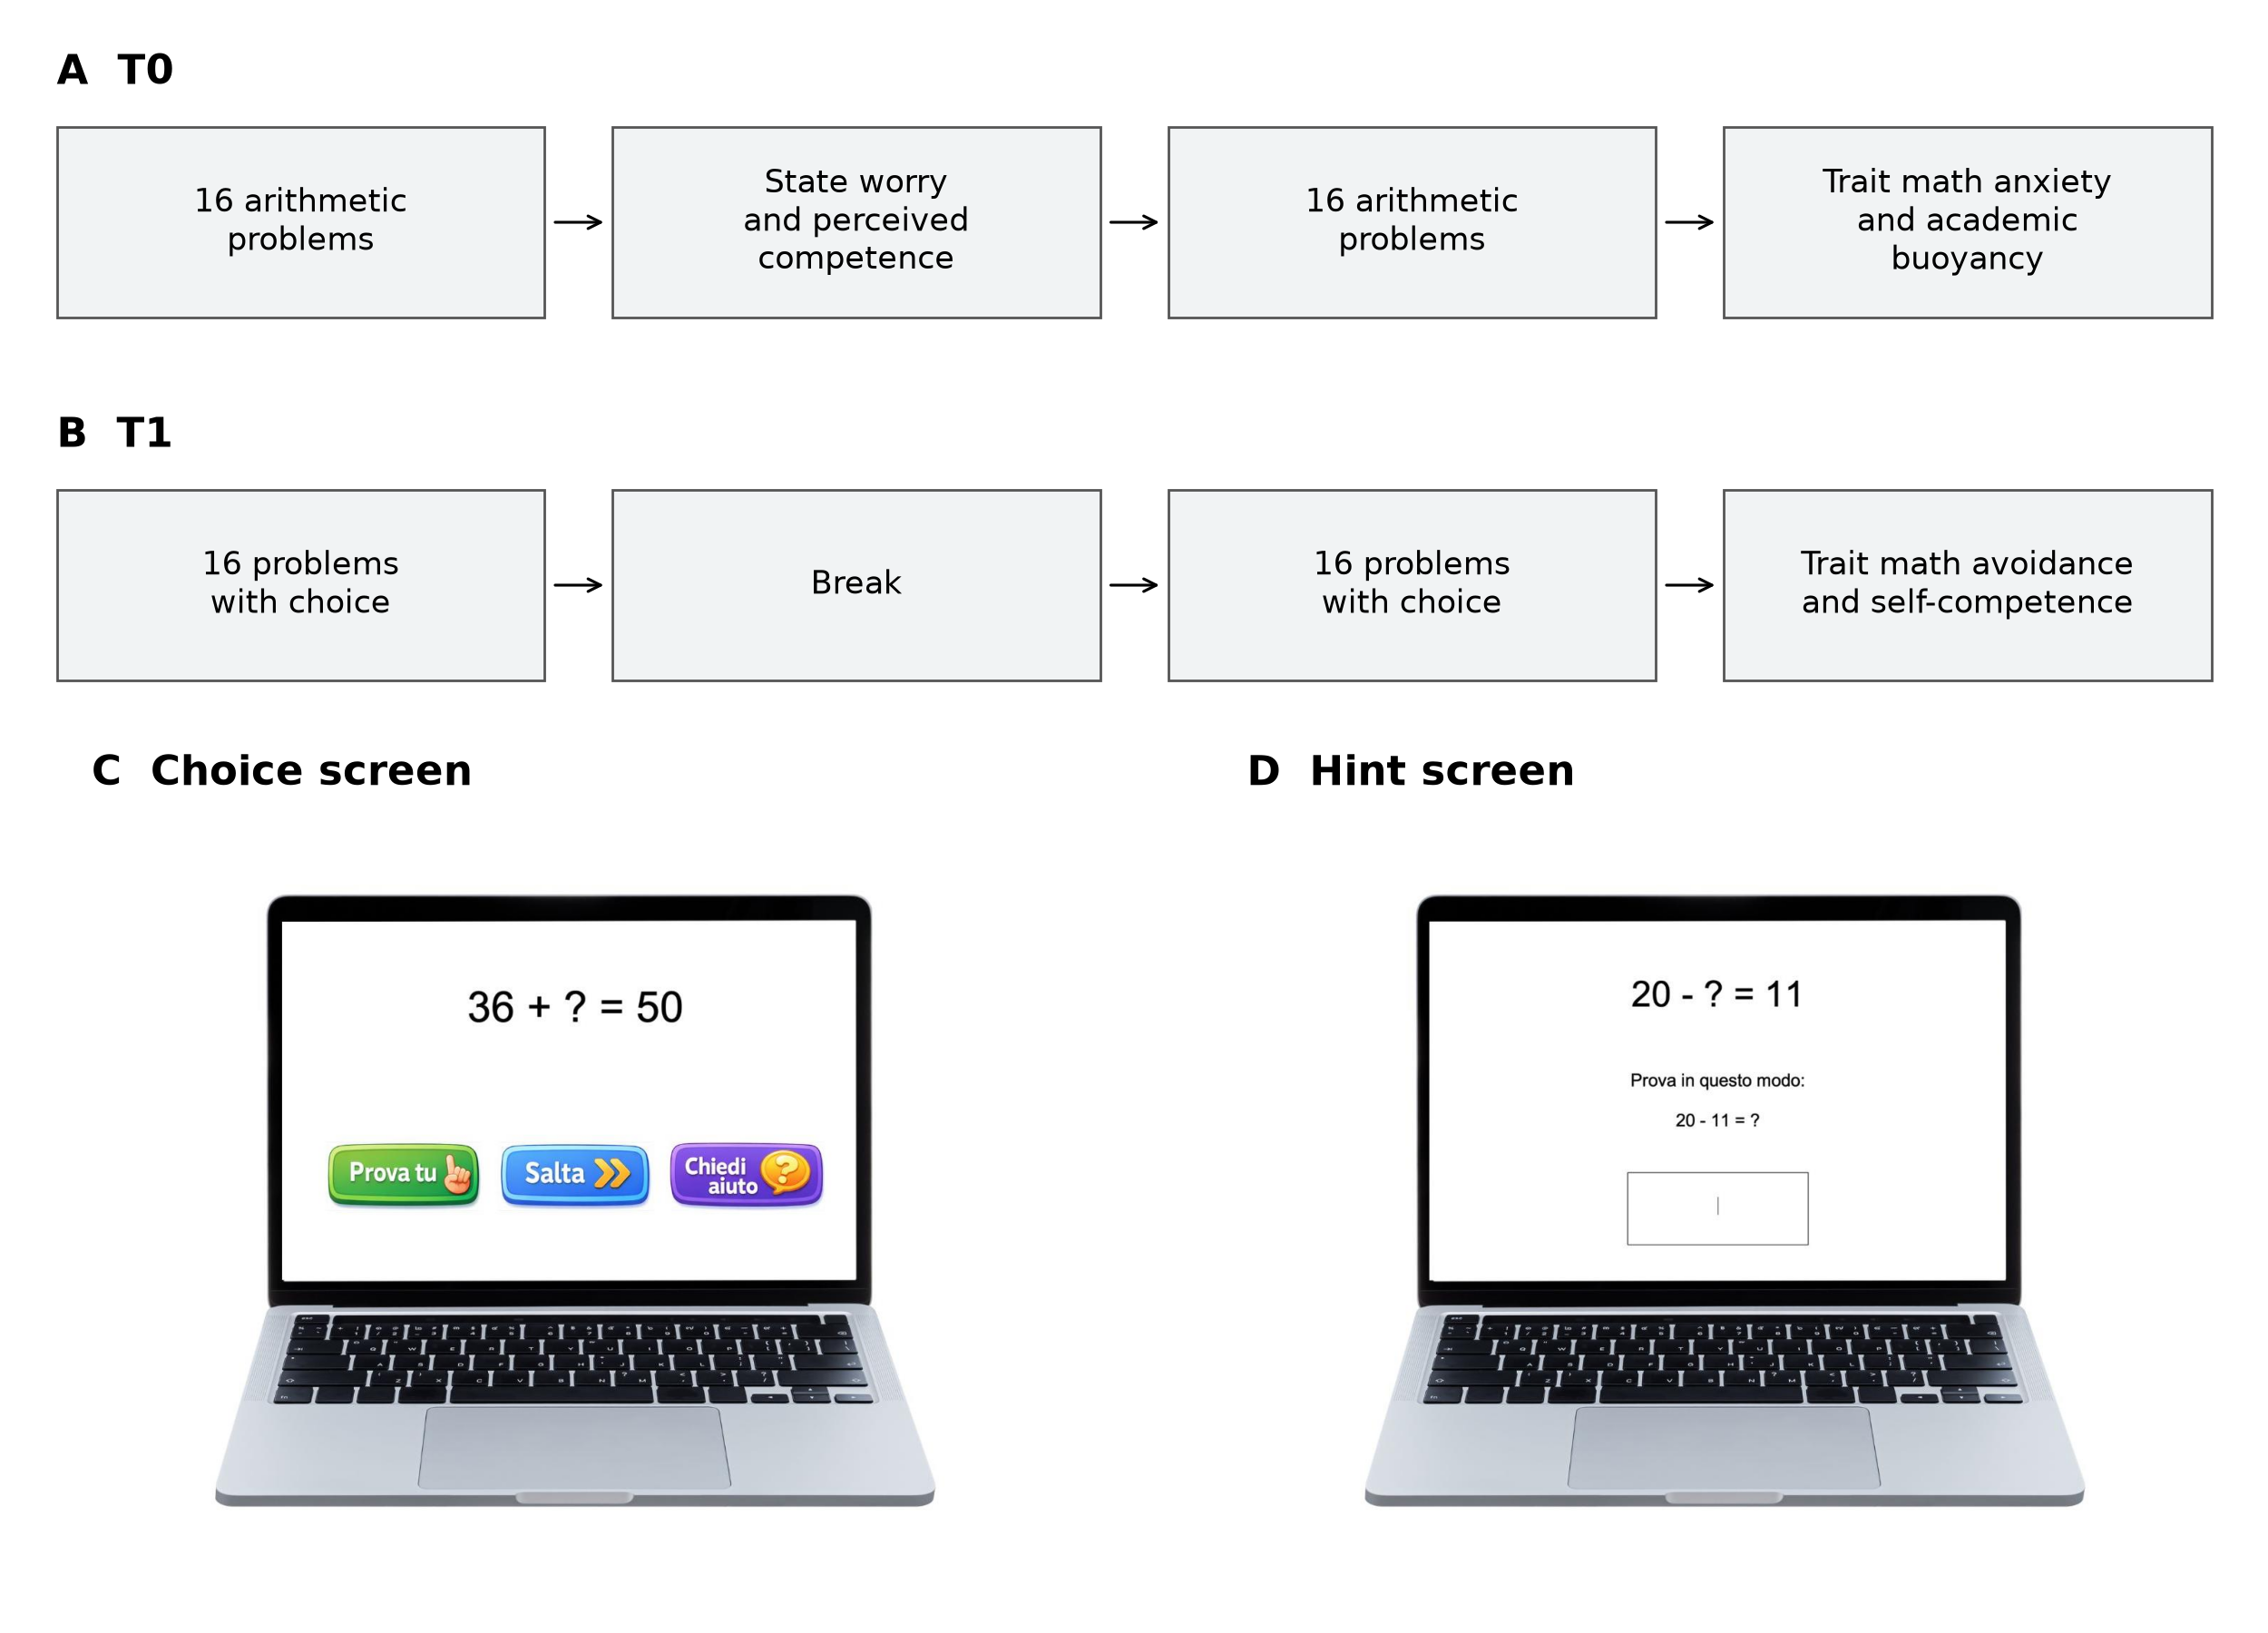
\includegraphics[width=1\linewidth,height=\textheight,keepaspectratio]{figures/fig_design.png}

}

\end{figure}%

\subsection{Measures}\label{measures}

\subsubsection{Math Task}\label{math-task}

A pool of 100 arithmetic problems with one unknown term (e.g., 34 − ? =
21) was generated with constraints: operands between 12 and 99, no
multiples of 10, and balanced position of the unknown term. For each
child, 32 problems per session were sampled at random, excluding at T1
the problems already presented at T0. Answers were typed on the
keyboard, with a time limit of 25 s per problem, set on the basis of a
pilot study. Correct and timely answers scored 1; incorrect, late, or
skipped answers scored 0. Prior math ability was the T0 total score
(0--32).

\subsubsection{Behavioural Choice}\label{behavioural-choice}

At T1, each problem was presented with three options: not solving it
(\emph{skip}), requesting a hint with a brief strategy (\emph{help};
e.g., for ``20 − ? = 11'': ``Try this way: 20 − 11 = ?''), or solving it
independently (\emph{self}). Two features discouraged extreme patterns:
a mandatory dwell time of 15 s per item after each choice, and an
automatic prompt after every 5 consecutive skips or help requests,
reminding children of all options. Skipped problems were not treated as
missing data: skipping is one category of the outcome. A choice was
coded as missing when all three choice indicators were missing in the
supplied export; these trials were excluded from the choice models.
\textbf{{[}TODO: confirm whether these records reflect timeouts before a
choice or another logging event; the export contains no timing or event
logs.{]}}

\subsubsection{Questionnaires}\label{questionnaires}

Scores were sums of items; higher scores mean more of the construct.
Responses were mandatory, so questionnaire data were complete.

\begin{itemize}
\tightlist
\item
  \emph{Math anxiety} (trait): Abbreviated Math Anxiety Scale
  (\citeproc{ref-caviola2017}{Caviola et al., 2017}), 9 items, 5-point
  scale.
\item
  \emph{Academic buoyancy} (trait): Academic Buoyancy Scale
  (\citeproc{ref-martin2008}{Martin \& Marsh, 2008}), 4 items, 7-point
  scale.
\item
  \emph{Math avoidance} (trait): adapted Math Avoidance Scale
  (\citeproc{ref-conlon2022}{Conlon et al., 2022}), 10 items, 4-point
  scale.
\item
  \emph{Math self-competence} (trait): adapted from Harter
  (\citeproc{ref-harter2012}{2012}), 10 items, 4-point scale.
\item
  \emph{Worry} and \emph{perceived competence} (state): 3 items each,
  adapted from Mammarella et al. (\citeproc{ref-mammarella2023}{2023}),
  4-point scale, referring to the problems just solved.
\end{itemize}

\subsection{Preregistration and
Deviations}\label{preregistration-and-deviations}

The study was preregistered while data collection was ongoing, before
any data were inspected. The preregistration, simulated data, power
analyses, and analysis script are available at \textbf{{[}TODO: OSF
link{]}}. Table~\ref{tbl-deviations} lists the deviations
(\citeproc{ref-willroth2024}{Willroth \& Atherton, 2024}).

\begin{table}

{\caption{{Deviations From the Preregistration}{\label{tbl-deviations}}}
\vspace{-20pt}}

\begin{longtable}[]{@{}
  >{\raggedright\arraybackslash}p{(\linewidth - 4\tabcolsep) * \real{0.3333}}
  >{\raggedright\arraybackslash}p{(\linewidth - 4\tabcolsep) * \real{0.3333}}
  >{\raggedright\arraybackslash}p{(\linewidth - 4\tabcolsep) * \real{0.3333}}@{}}
\toprule\noalign{}
\begin{minipage}[b]{\linewidth}\raggedright
Preregistered
\end{minipage} & \begin{minipage}[b]{\linewidth}\raggedright
What we did
\end{minipage} & \begin{minipage}[b]{\linewidth}\raggedright
Reason
\end{minipage} \\
\midrule\noalign{}
\endhead
\bottomrule\noalign{}
\endlastfoot
Ordinal (cumulative) model; categorical model only as follow-up if the
ordinal structure proved clearly inadequate & Ordinal models reported in
full; multinomial model used as the main model for RQ1 & The data did
not support the ordinal structure (see Assumption Check) \\
Predictors selected by LOO within the ordinal model (M0 → M1 → M2) &
Multinomial model with all predictors & The selection was conducted
within the ordinal model; trial-level LOO evaluates prediction for
already-observed children (see Results) \\
Pragmatic frequentist inference (one-tailed \emph{p}, FDR) & Kept for
the ordinal models; follow-up models reported with posterior estimates
and 95\% credible intervals & Follow-up analyses are exploratory \\
Indirect effects (trait → state → choice) & Reported for the ordinal
models only & Order of measurement does not support a mediation reading
(see Limitations) \\
--- & Robustness: linear model on a per-child choice score; class random
intercept; binary models & Not anticipated \\
A construct failing CFA screening excluded from all models & Avoidance
excluded from the ordinal pipeline but retained in exploratory follow-up
models & Scaled CFI = .923; follow-up estimates allow its association
with each choice to be examined, with this measurement limitation \\
\end{longtable}

\end{table}

\subsection{Statistical Analyses}\label{statistical-analyses}

Analyses were run in R 4.5.1. Bayesian models were estimated with brms
2.22.0 (\citeproc{ref-burkner2017}{Bürkner, 2017}) and the RStan
backend, using 4 chains of 2000 iterations, including 1000 warmup
iterations per chain (seed 2026). We used brms default priors: flat
priors on choice-model regression coefficients, Student's \emph{t}(3, 0,
2.5) priors on intercepts, and the corresponding half-\emph{t} priors on
random-effect standard deviations. All continuous predictors were
standardised across children. All choice models included a random
intercept for participant. Models were compared with Pareto-smoothed
leave-one-out cross-validation (PSIS-LOO,
\citeproc{ref-vehtari2017}{Vehtari et al., 2017}). A difference in
expected log predictive density (ELPD) larger than twice its standard
error was taken as a clear preference.

Models were fitted to counts per child and choice, with counts used as
likelihood weights. This gives the same likelihood as the trial-level
data. For LOO, weighted log likelihoods were divided by the counts and
the resulting pointwise estimates repeated for the corresponding trials.
Thus, LOO left out one trial, with the child's other trials available;
it did not evaluate prediction for a new child. Full posterior draws
were used for inference and then discarded; only numerical summaries,
diagnostics and predictions were retained.

\subsubsection{Psychometric Screening}\label{psychometric-screening}

We fitted a confirmatory factor analysis (CFA) for buoyancy and for
avoidance (criteria: CFI \textgreater{} .95, RMSEA \textless{} .08),
using WLSMV estimation and the scaled fit indices. The preregistration
did not specify scaled or unscaled indices; we used the scaled ones
consistently in the ordinal pipeline. If a model did not meet the
criteria, at most two correlated residuals could be added, only between
items with clear overlap in content or wording. No correlated residuals
were added. A construct still failing was excluded from the ordinal
pipeline; its inclusion in follow-up models was exploratory
(Table~\ref{tbl-deviations}). Ordinal alpha was computed as a
descriptive index, not as a pass/fail criterion. If buoyancy and
avoidance correlated above \textbar{}\emph{r}\textbar{} = .70, they were
not to be entered in the same model.

\subsubsection{Ordinal Models}\label{ordinal-models}

Choices were modelled with cumulative logit mixed models
(\citeproc{ref-burkner2019}{Bürkner \& Vuorre, 2019}), ordered as skip
\textless{} help \textless{} self. In Stage 1, the baseline model (M0)
included the state predictors (worry and perceived competence), the
covariates (prior math ability and gender), and a random intercept for
participant; this is the full mediation model. M1 added predictors
passing screening (buoyancy in this run). M2 added math anxiety and
self-competence (partial mediation), and was to be estimated only if M1
was preferred over M0. In Stage 2, category-specific effects were added
to the selected model one predictor at a time, in the order worry,
perceived competence, buoyancy, avoidance, restricted to retained
predictors. At each step, the more complex model was retained only if
clearly preferred; otherwise the simpler model was kept and selection
stopped.

As preregistered, inference on the final model was pragmatically
frequentist: MCMC served to estimate coefficients and their standard
errors, not for Bayesian inference. Primary directional effects were
tested with one-tailed \emph{p}-values computed from the posterior mean
and standard deviation, with FDR correction across the primary effects
retained (\citeproc{ref-benjamini1995}{Benjamini \& Hochberg, 1995}).
Positive coefficients were expected for buoyancy and perceived
competence, negative coefficients for avoidance and worry. Indirect
effects were computed by multiplying posterior draws of the trait →
state paths, from regressions of each state measure on its trait
counterpart, by those of the state → choice paths.

\subsubsection{Assumption Check}\label{assumption-check}

We checked the ordinal assumption in three ways: (a) within the ordinal
models, by testing category-specific effects (RQ2); (b) by comparing,
via LOO, the cumulative model with a multinomial model that imposes no
order, both including all predictors; (c) descriptively, by comparing
how the proportions of each choice correlate with the predictors.

\subsubsection{Multinomial Model}\label{multinomial-model}

Choices were modelled with a multinomial logit mixed model with skip as
the reference category, including state and trait predictors and
controlling for math ability and gender.

\subsubsection{Robustness}\label{robustness}

\begin{enumerate}
\def\labelenumi{(\alph{enumi})}
\tightlist
\item
  A frequentist linear regression on a per-child sum of valid choices
  (skip = 0, help = 1, self = 2; standardised), with the same
  predictors, and the same regression on the proportion of self choices,
  which assumes no order between skip and help; (b) a random intercept
  for class; (c) binary mixed logistic models {[}lme4; Bates et al.
  (\citeproc{ref-bates2015}{2015}){]} with random intercepts for child,
  class, and item, for self vs not self, skip vs not skip, and skip vs
  help (trials without self choice), entering all predictors together or
  one attitude at a time (plus ability and gender). Binary models with
  only the child intercept provided a further comparison.
\end{enumerate}

\section{Results}\label{results}

\subsection{Descriptive Statistics}\label{descriptive-statistics}

Table~\ref{tbl-desc} reports the descriptive statistics of the
predictors, and Table~\ref{tbl-gender} reports them by gender and grade.
In both grades, girls reported higher math anxiety and worry, and lower
self-competence, perceived competence, and buoyancy than boys; they also
had lower T0 ability, by about four points. Grade 5 children had higher
T0 ability than Grade 4 children, also by about four points, but similar
attitudes. Correlations are reported in Table~\ref{tbl-cor}. Trait and
state measures showed good convergent validity: math anxiety and worry
(\emph{r} = .50) and self-competence and perceived competence (\emph{r}
= .36) were correlated but not redundant. Buoyancy was related to the
other variables as expected.

\begin{table}

{\caption{{Descriptive Statistics of the Predictors}{\label{tbl-desc}}}
\vspace{-20pt}}

\begin{longtable}[]{@{}
  >{\raggedright\arraybackslash}p{(\linewidth - 10\tabcolsep) * \real{0.4265}}
  >{\raggedleft\arraybackslash}p{(\linewidth - 10\tabcolsep) * \real{0.1912}}
  >{\raggedleft\arraybackslash}p{(\linewidth - 10\tabcolsep) * \real{0.0588}}
  >{\raggedleft\arraybackslash}p{(\linewidth - 10\tabcolsep) * \real{0.0588}}
  >{\raggedleft\arraybackslash}p{(\linewidth - 10\tabcolsep) * \real{0.1324}}
  >{\raggedleft\arraybackslash}p{(\linewidth - 10\tabcolsep) * \real{0.1324}}@{}}
\toprule\noalign{}
\begin{minipage}[b]{\linewidth}\raggedright
Variable
\end{minipage} & \begin{minipage}[b]{\linewidth}\raggedleft
M (SD)
\end{minipage} & \begin{minipage}[b]{\linewidth}\raggedleft
Min
\end{minipage} & \begin{minipage}[b]{\linewidth}\raggedleft
Max
\end{minipage} & \begin{minipage}[b]{\linewidth}\raggedleft
Skewness
\end{minipage} & \begin{minipage}[b]{\linewidth}\raggedleft
Kurtosis
\end{minipage} \\
\midrule\noalign{}
\endhead
\bottomrule\noalign{}
\endlastfoot
Worry (state) & 5.50 (2.06) & 3 & 12 & 0.90 & 0.23 \\
Perceived competence (state) & 8.36 (2.31) & 3 & 12 & -0.42 & -0.38 \\
Math anxiety (trait) & 22.26 (7.57) & 9 & 44 & 0.16 & -0.64 \\
Self-competence (trait) & 27.04 (5.96) & 10 & 40 & 0.21 & -0.53 \\
Academic buoyancy & 19.27 (4.90) & 4 & 28 & -0.34 & -0.08 \\
Math avoidance & 17.69 (5.26) & 10 & 40 & 1.12 & 1.70 \\
Math ability (T0) & 11.77 (7.90) & 0 & 32 & 0.45 & -0.77 \\
\end{longtable}

\vspace{-20pt}
\noindent \emph{Note.} Raw~scores; \emph{N} = 547.

\end{table}

\begin{table}

{\caption{{Descriptive Statistics by Gender and
Grade}{\label{tbl-gender}}}
\vspace{-20pt}}

\begin{longtable}[]{@{}
  >{\raggedright\arraybackslash}p{(\linewidth - 8\tabcolsep) * \real{0.2710}}
  >{\raggedleft\arraybackslash}p{(\linewidth - 8\tabcolsep) * \real{0.1869}}
  >{\raggedleft\arraybackslash}p{(\linewidth - 8\tabcolsep) * \real{0.1869}}
  >{\raggedleft\arraybackslash}p{(\linewidth - 8\tabcolsep) * \real{0.1776}}
  >{\raggedleft\arraybackslash}p{(\linewidth - 8\tabcolsep) * \real{0.1776}}@{}}
\toprule\noalign{}
\begin{minipage}[b]{\linewidth}\raggedright
Variable
\end{minipage} & \begin{minipage}[b]{\linewidth}\raggedleft
Grade 4 F (n = 207)
\end{minipage} & \begin{minipage}[b]{\linewidth}\raggedleft
Grade 4 M (n = 171)
\end{minipage} & \begin{minipage}[b]{\linewidth}\raggedleft
Grade 5 F (n = 90)
\end{minipage} & \begin{minipage}[b]{\linewidth}\raggedleft
Grade 5 M (n = 79)
\end{minipage} \\
\midrule\noalign{}
\endhead
\bottomrule\noalign{}
\endlastfoot
Worry (state) & 6.10 (2.03) & 4.94 (1.78) & 5.83 (2.35) & 4.77 (1.80) \\
Perceived competence (state) & 7.65 (2.21) & 9.11 (2.01) & 7.69 (2.23) &
9.34 (2.45) \\
Math anxiety (trait) & 24.01 (7.27) & 20.71 (7.95) & 23.12 (6.76) &
20.06 (7.23) \\
Self-competence (trait) & 26.26 (5.52) & 27.85 (5.78) & 25.99 (6.18) &
28.56 (6.74) \\
Academic buoyancy & 18.67 (4.63) & 20.05 (5.20) & 18.41 (4.67) & 20.10
(4.87) \\
Math avoidance & 17.31 (4.88) & 17.55 (5.53) & 18.17 (4.72) & 18.48
(6.10) \\
Math ability (T0) & 8.62 (6.43) & 12.55 (7.69) & 12.97 (7.91) & 16.95
(8.40) \\
\end{longtable}

\vspace{-20pt}
\noindent \emph{Note.} \emph{M}~(\emph{SD}) of raw scores. F = girls; M
= boys.

\end{table}

\begin{table}

{\caption{{Pearson Correlations Among the Predictors}{\label{tbl-cor}}}
\vspace{-20pt}}

\begin{longtable}[]{@{}lrrrrrr@{}}
\toprule\noalign{}
Variable & 1 & 2 & 3 & 4 & 5 & 6 \\
\midrule\noalign{}
\endhead
\bottomrule\noalign{}
\endlastfoot
1. Worry (state) & & & & & & \\
2. Perceived competence (state) & -.57 & & & & & \\
3. Math anxiety (trait) & .50 & -.42 & & & & \\
4. Self-competence (trait) & -.25 & .36 & -.38 & & & \\
5. Academic buoyancy & -.39 & .46 & -.44 & .35 & & \\
6. Math avoidance & .19 & -.25 & .38 & -.35 & -.33 & \\
7. Math ability (T0) & -.30 & .44 & -.37 & .26 & .30 & -.22 \\
\end{longtable}

\end{table}

Children chose to solve alone in 59.2\% of all trials, asked for help in
30.3\%, and skipped in 8.3\%. Among valid choices, block proportions
were similar (skip: 7.6\% and 9.4\%; help: 31.9\% and 30.1\%; self:
60.5\% in both). Patterns varied across children: 57 always solved
alone, 3 always asked for help, and none always skipped. Skipping was
concentrated in a minority of children: 215 never skipped, and the
median child skipped 3\% of the problems; 78 children never asked for
help. Choices were missing in 2.1\% of trials (363 trials); 363 children
had no missing choice, and none had more than 10. All trials with a
missing choice already had accuracy coded as 0 in the supplied export.
Accuracy was low: 26.7\% after self and 27.5\% after help. Controlling
for T0 ability, accuracy was higher after help than after self (logit
difference = 0.47, \emph{SE} = 0.05). This comparison is observational,
because children chose whether to request help.

\subsection{Psychometric Screening}\label{psychometric-screening-1}

The CFA for buoyancy fitted well (scaled CFI = .998, RMSEA = .030;
standardised loadings .51--.77; ordinal alpha = .70, ordinal omega =
.67). For avoidance, the RMSEA criterion was met (scaled RMSEA = .078),
but the scaled CFI (.923) was below the .95 threshold; the unscaled CFI
was .971 (standardised loadings .47--.72; ordinal alpha = .84, ordinal
omega = .79). We therefore excluded avoidance from the ordinal pipeline.
It was retained in the exploratory follow-up models, so its associations
require caution given the imperfect unidimensional fit. The
buoyancy--avoidance correlation (\emph{r} = −.33) was well below .70.

\subsection{Ordinal Models}\label{ordinal-models-1}

M1, adding buoyancy, did not clearly improve on M0 (ΔELPD = 0.28,
\emph{SE} = 0.70). Following the selection rule, M0 was retained and M2
was not estimated. Avoidance had already been excluded by screening. In
Stage 2, a category-specific effect of worry was clearly preferred
(ΔELPD = 21.81, \emph{SE} = 7.24). Extending perceived competence as
well did not improve prediction (ΔELPD = -0.24, \emph{SE} = 1.91), so
selection stopped.

In the final model (Table~\ref{tbl-prereg}), worry was unrelated to the
first threshold (skip vs help or self) and negatively related to the
second (skip or help vs self). Perceived competence was unrelated to
choice. The indirect effect of math anxiety via worry was credible only
on the second threshold.

\begin{table}

{\caption{{Final Ordinal Model}{\label{tbl-prereg}}}
\vspace{-20pt}}

\begin{longtable}[]{@{}
  >{\raggedright\arraybackslash}p{(\linewidth - 8\tabcolsep) * \real{0.4659}}
  >{\raggedleft\arraybackslash}p{(\linewidth - 8\tabcolsep) * \real{0.1023}}
  >{\raggedleft\arraybackslash}p{(\linewidth - 8\tabcolsep) * \real{0.1705}}
  >{\raggedleft\arraybackslash}p{(\linewidth - 8\tabcolsep) * \real{0.1705}}
  >{\raggedleft\arraybackslash}p{(\linewidth - 8\tabcolsep) * \real{0.0909}}@{}}
\toprule\noalign{}
\begin{minipage}[b]{\linewidth}\raggedright
Parameter
\end{minipage} & \begin{minipage}[b]{\linewidth}\raggedleft
Estimate
\end{minipage} & \begin{minipage}[b]{\linewidth}\raggedleft
95\% interval
\end{minipage} & \begin{minipage}[b]{\linewidth}\raggedleft
p (one-tailed)
\end{minipage} & \begin{minipage}[b]{\linewidth}\raggedleft
p (FDR)
\end{minipage} \\
\midrule\noalign{}
\endhead
\bottomrule\noalign{}
\endlastfoot
Worry, first threshold & -0.02 & {[}-0.17, 0.14{]} & .406 & .430 \\
Worry, second threshold & -0.23 & {[}-0.38, -0.08{]} & .001 & .003 \\
Perceived competence & 0.01 & {[}-0.14, 0.16{]} & .430 & .430 \\
Anxiety via worry, first threshold & -0.01 & {[}-0.08, 0.06{]} & .407 &
.431 \\
Anxiety via worry, second threshold & -0.10 & {[}-0.17, -0.04{]} & .001
& .004 \\
Self-competence via perceived competence & 0.00 & {[}-0.03, 0.04{]} &
.431 & .431 \\
\end{longtable}

\vspace{-20pt}
\noindent \emph{Note.} Cumulative~logit mixed model with a
category-specific effect of worry. Positive values indicate more engaged
choices.

\end{table}

The failure to retain buoyancy is a predictive selection result, not
evidence of no association. With trial-level LOO, a child's random
intercept is informed by their remaining valid trials. Predictors
varying only between children may therefore add little to prediction for
that child. In the exploratory full cumulative model, buoyancy and
avoidance both had negative coefficients. The screening decision for
avoidance and the LOO decision for buoyancy are distinct.

\subsection{Assumption Check: Are the Choices
Ordinal?}\label{assumption-check-are-the-choices-ordinal}

The categorical model was clearly preferred over the full cumulative
model (ΔELPD = -718.8, \emph{SE} = 35.9 for the cumulative model), with
a difference of about 20 \emph{SE}, well beyond the 2 \emph{SE}
threshold. The adjacent-category model with category-specific effects
also predicted less well than the categorical model (ΔELPD = -847.3,
\emph{SE} = 39.2). The data therefore did not support the ordinal
specifications examined here.

The proportional-odds model assumes that each predictor has the same
effect on both thresholds of the choice (skip vs help + self, and skip +
help vs self). The data showed non-proportional patterns. The ordinal
pipeline had already required a category-specific effect of worry. In
the adjacent-category model, worry was associated with more help
relative to skip (0.16 {[}0.01, 0.30{]}) and with less self relative to
help (-0.29 {[}-0.42, -0.17{]}). A single proportional effect cannot
describe a predictor that moves children towards the middle category.
Non-proportionality alone does not rule out an order, but it helps
explain why a simple engagement score is inadequate here.

Descriptively, the proportions of skip and help choices correlated with
the predictors in a similar way, and the proportion of self choices in
the opposite way (Table~\ref{tbl-bivar}). The main contrast is between
solving alone and not solving alone; help does not appear to lie between
skip and self.

\begin{table}

{\caption{{Correlations Between Each Child's Proportion of Choices and
the Predictors}{\label{tbl-bivar}}}
\vspace{-20pt}}

\begin{longtable}[]{@{}
  >{\raggedright\arraybackslash}p{(\linewidth - 14\tabcolsep) * \real{0.0921}}
  >{\raggedleft\arraybackslash}p{(\linewidth - 14\tabcolsep) * \real{0.0789}}
  >{\raggedleft\arraybackslash}p{(\linewidth - 14\tabcolsep) * \real{0.1579}}
  >{\raggedleft\arraybackslash}p{(\linewidth - 14\tabcolsep) * \real{0.1711}}
  >{\raggedleft\arraybackslash}p{(\linewidth - 14\tabcolsep) * \real{0.1447}}
  >{\raggedleft\arraybackslash}p{(\linewidth - 14\tabcolsep) * \real{0.1184}}
  >{\raggedleft\arraybackslash}p{(\linewidth - 14\tabcolsep) * \real{0.1316}}
  >{\raggedleft\arraybackslash}p{(\linewidth - 14\tabcolsep) * \real{0.1053}}@{}}
\toprule\noalign{}
\begin{minipage}[b]{\linewidth}\raggedright
Choice
\end{minipage} & \begin{minipage}[b]{\linewidth}\raggedleft
Worry
\end{minipage} & \begin{minipage}[b]{\linewidth}\raggedleft
Perc. comp.
\end{minipage} & \begin{minipage}[b]{\linewidth}\raggedleft
Math anxiety
\end{minipage} & \begin{minipage}[b]{\linewidth}\raggedleft
Self-comp.
\end{minipage} & \begin{minipage}[b]{\linewidth}\raggedleft
Buoyancy
\end{minipage} & \begin{minipage}[b]{\linewidth}\raggedleft
Avoidance
\end{minipage} & \begin{minipage}[b]{\linewidth}\raggedleft
Ability
\end{minipage} \\
\midrule\noalign{}
\endhead
\bottomrule\noalign{}
\endlastfoot
Skip & .12 & -.21 & .16 & -.15 & -.09 & .21 & -.40 \\
Help & .26 & -.22 & .19 & -.13 & -.10 & .14 & -.41 \\
Self & -.27 & .27 & -.22 & .17 & .12 & -.20 & .50 \\
\end{longtable}

\vspace{-20pt}
\noindent \emph{Note.} Perc.~comp. = perceived competence (state);
Self-comp. = self-competence (trait).

\end{table}

The categorical model therefore guided all subsequent analyses.

\subsection{Multinomial Model}\label{multinomial-model-1}

Table~\ref{tbl-multi} reports the multinomial model;
Figure~\ref{fig-pred} shows predicted probabilities. Math ability was by
far the strongest predictor of solving alone. Among attitudes:

\begin{itemize}
\tightlist
\item
  \textbf{Avoidance} was associated with fewer self-reliant responses
  relative to skipping (-0.27 {[}-0.43, -0.11{]}) and, less clearly,
  with fewer help requests relative to skipping (-0.12 {[}-0.26,
  0.03{]}; posterior probability of a negative effect = 0.94).
\item
  \textbf{Worry} was associated with more help requests relative to
  skipping (0.26 {[}0.08, 0.42{]}), but not with self-reliant responding
  relative to skipping (-0.10 {[}-0.29, 0.09{]}). The derived contrast
  self vs help was -0.36 {[}-0.57, -0.14{]}: worry was associated with
  help-seeking relative to both alternatives.
\item
  \textbf{Buoyancy} was associated with fewer self-reliant responses
  relative to skipping (-0.20 {[}-0.38, -0.03{]}), opposite to what we
  expected.
\item
  Perceived competence (state and trait), math anxiety, and gender were
  not credible predictors.
\end{itemize}

\begin{table}

{\caption{{Multinomial Logit Mixed Model of the Behavioural
Choice}{\label{tbl-multi}}}
\vspace{-20pt}}

\begin{longtable}[]{@{}
  >{\raggedright\arraybackslash}p{(\linewidth - 6\tabcolsep) * \real{0.3187}}
  >{\raggedleft\arraybackslash}p{(\linewidth - 6\tabcolsep) * \real{0.2198}}
  >{\raggedleft\arraybackslash}p{(\linewidth - 6\tabcolsep) * \real{0.2308}}
  >{\raggedleft\arraybackslash}p{(\linewidth - 6\tabcolsep) * \real{0.2308}}@{}}
\toprule\noalign{}
\begin{minipage}[b]{\linewidth}\raggedright
Predictor
\end{minipage} & \begin{minipage}[b]{\linewidth}\raggedleft
Help vs skip
\end{minipage} & \begin{minipage}[b]{\linewidth}\raggedleft
Self vs skip
\end{minipage} & \begin{minipage}[b]{\linewidth}\raggedleft
Self vs help
\end{minipage} \\
\midrule\noalign{}
\endhead
\bottomrule\noalign{}
\endlastfoot
Worry (state) & 0.26 {[}0.08, 0.42{]} & -0.10 {[}-0.29, 0.09{]} & -0.36
{[}-0.57, -0.14{]} \\
Perceived competence (state) & 0.04 {[}-0.12, 0.22{]} & 0.05 {[}-0.15,
0.25{]} & 0.01 {[}-0.22, 0.24{]} \\
Math anxiety (trait) & -0.05 {[}-0.21, 0.12{]} & 0.02 {[}-0.17, 0.20{]}
& 0.07 {[}-0.15, 0.28{]} \\
Self-competence (trait) & 0.01 {[}-0.14, 0.16{]} & 0.04 {[}-0.13,
0.21{]} & 0.03 {[}-0.16, 0.23{]} \\
Academic buoyancy & -0.01 {[}-0.17, 0.14{]} & -0.20 {[}-0.38, -0.03{]} &
-0.19 {[}-0.40, 0.02{]} \\
Math avoidance & -0.12 {[}-0.26, 0.03{]} & -0.27 {[}-0.43, -0.11{]} &
-0.15 {[}-0.34, 0.05{]} \\
Math ability (T0) & 0.12 {[}-0.03, 0.28{]} & 1.08 {[}0.90, 1.25{]} &
0.95 {[}0.75, 1.15{]} \\
Gender (boys) & 0.09 {[}-0.18, 0.37{]} & 0.00 {[}-0.30, 0.33{]} & -0.08
{[}-0.45, 0.28{]} \\
\end{longtable}

\vspace{-20pt}
\noindent \emph{Note.} Reference~category = skip. Estimates on the logit
scale with 95\% credible intervals; continuous predictors standardised.

\end{table}

\begin{figure}[h]

\caption{\label{fig-pred}Predicted Probability of Each Choice as a
Function of Selected Predictors}

\centering{

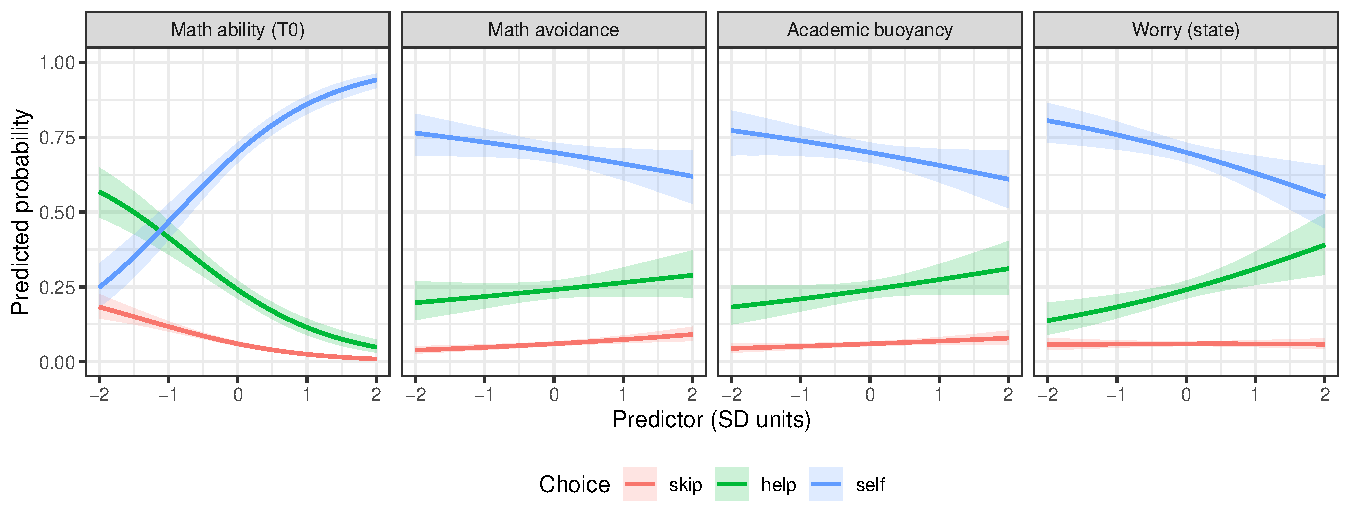
\includegraphics[width=1\linewidth,height=\textheight,keepaspectratio]{../analysis/figures/fig_pred.pdf}

}

\end{figure}%

In Figure~\ref{fig-pred}, other continuous predictors are held at their
means, participant intercepts are set to zero, and predictions are
averaged over gender in the sample. Bands show 95\% credible intervals.

Compared with our initial hypotheses, avoidance behaved as expected.
Worry was expected to increase skipping; it was associated with
help-seeking instead. Perceived competence showed no clear association,
and buoyancy went in the opposite direction. Across global parameters of
the Bayesian models, the largest Rhat was 1.016, the smallest bulk ESS
was 398, and the smallest tail ESS was 272. There were no divergent
transitions and no trial-level Pareto \emph{k} values above .70 in the
LOO comparisons.

\subsection{Robustness}\label{robustness-1}

\subsubsection{Linear Model}\label{linear-model}

In the linear regression on the per-child choice score
(Table~\ref{tbl-lm}), math ability was the strongest predictor, and
worry, avoidance, and buoyancy were associated with lower scores,
confirming the picture from the multinomial model. This score assumes
the ordering skip \textless{} help \textless{} self, so it is only a
coarse check of the direction of effects. The same pattern held for the
proportion of self choices, which assumes no order between skip and
help: ability β = 0.47, worry β = −0.17, buoyancy β = −0.11, avoidance β
= −0.10 (all \emph{p} ≤ .021); no other predictor had \emph{p}
\textless{} .40.

\begin{table}

{\caption{{Linear Regression on the Per-Child Choice
Score}{\label{tbl-lm}}}
\vspace{-20pt}}

\begin{longtable}[]{@{}lrrr@{}}
\toprule\noalign{}
Predictor & beta & 95\% CI & p \\
\midrule\noalign{}
\endhead
\bottomrule\noalign{}
\endlastfoot
Math ability (T0) & 0.51 & {[}0.43, 0.59{]} & \textless{} .001 \\
Worry (state) & -0.13 & {[}-0.22, -0.04{]} & .005 \\
Academic buoyancy & -0.11 & {[}-0.20, -0.03{]} & .008 \\
Math avoidance & -0.10 & {[}-0.18, -0.02{]} & .013 \\
Self-competence (trait) & 0.03 & {[}-0.05, 0.11{]} & .437 \\
Perceived competence (state) & 0.04 & {[}-0.06, 0.13{]} & .470 \\
Math anxiety (trait) & 0.02 & {[}-0.07, 0.11{]} & .676 \\
Gender (boys) & -0.05 & {[}-0.20, 0.10{]} & .506 \\
\end{longtable}

\vspace{-20pt}
\noindent \emph{Note.} Choice~score: skip = 0, help = 1, self = 2,
summed over the 32 trials and standardised. \emph{R}² = .331 (adjusted
\emph{R}² = .321), \emph{F}(8, 538) = 33.32, \emph{p} \textless{} .001.

\end{table}

\subsubsection{Class and Item Random
Intercepts}\label{class-and-item-random-intercepts}

Adding a random intercept for class to the multinomial model (\emph{SD}
= 0.37 for help vs skip, 0.49 for self vs skip) left estimates
practically unchanged (largest absolute change: 0.06, for gender in help
vs skip). In the binary models, the item intercept also varied
(\emph{SD} = 0.41 for self vs not self): problems differed in how often
children chose to solve them alone. Adding class and item intercepts to
models with only the child intercept changed the attitude estimates by
0.04 at most. No binary model was singular or produced a convergence
warning.

\subsubsection{Skip vs Help}\label{skip-vs-help}

Among trials in which children did not choose to solve alone, worry was
associated with asking for help rather than skipping (skip vs help:
\emph{b} = -0.29, \emph{SE} = 0.09, \emph{p} = .002), and avoidance with
skipping rather than asking for help (\emph{b} = 0.17, \emph{SE} = 0.08,
\emph{p} = .033); higher ability was also associated with help rather
than skipping (\emph{b} = -0.30, \emph{SE} = 0.09, \emph{p} = .002).
Worry also predicted fewer self choices (self vs not self: \emph{b} =
-0.30, \emph{p} = .001). Avoidance predicted more skipping (skip vs not
skip: \emph{b} = 0.23, \emph{p} = .002), but its association with self
vs not self was less certain in the full model (\emph{b} = -0.14,
\emph{p} = .076). Thus, the binary models support the distinction
between worry and avoidance, with some uncertainty across contrasts.

\subsubsection{Buoyancy}\label{buoyancy}

The negative association of buoyancy appears only when the other
attitudes are controlled. At the bivariate level, buoyancy correlated
positively with the proportion of self choices (\emph{r} = .12;
Table~\ref{tbl-bivar}). In binary models of self vs not self, buoyancy
was unrelated to choice when entered alone with ability and gender
(\emph{b} = -0.03, \emph{SE} = 0.08, \emph{p} = .656), and negative only
with all attitudes in the model (\emph{b} = -0.18, \emph{SE} = 0.09,
\emph{p} = .035). This is consistent with suppression: buoyancy has
absolute correlations of .30 to .46 with worry, perceived competence,
math anxiety, and ability, and the negative coefficient refers to the
part of buoyancy not shared with them. Variance inflation factors were
modest (1.28--1.86). Avoidance, in contrast, gave similar estimates
alone and in the full model (self vs not self: -0.15 and -0.14; skip vs
not skip: 0.22 and 0.23), although the full-model association with self
choice was imprecise.

\section{Discussion}\label{discussion}

In our data, skipping, asking for help, and solving alone behaved more
like distinct categories than like levels of a single continuum of
engagement. Asking for help and skipping were related to the predictors
in a similar way, and both differed from solving alone. We initially
hypothesised that the choices were ordered, although we had planned a
categorical analysis in case they were not.

This has a methodological consequence. Behavioural categories that seem
ordered are often modelled as ordinal or converted into scores. Here, a
single ordinal coefficient would have masked the association of worry
with help relative to both alternatives. The category-specific extension
captured part of this pattern, but the categorical model predicted
choices much better. Avoidance was excluded by the psychometric screen,
whereas buoyancy was not retained by the ordinal model's predictive
selection rule. These decisions should not be confused with the absence
of an association. Whether behavioural categories are adequately
represented by an ordinal model is therefore worth testing rather than
assuming.

Math ability was by far the strongest predictor. Much of what looks like
avoidance of a single problem may be a realistic judgement that the
problem is too difficult, and problems differed in how often children
chose to solve them alone. The attitude effects are estimated net of
ability, and they were small: the credible ones were between 0.20 and
0.27 on the logit scale per \emph{SD} (odds ratios of about 0.76--1.28),
in the range assumed in the power analysis, whereas one \emph{SD} of
ability almost tripled the odds of solving alone rather than skipping.

Among trait attitudes, avoidance showed the clearest association with
choice. It was associated with fewer self-reliant responses and, less
clearly, fewer help requests relative to skipping. Binary models
supported its association with skipping, although the full-model
association with self vs not self was less certain. These results also
need caution because avoidance failed the scaled CFA criterion. State
worry, instead, was associated specifically with help-seeking: among the
problems children did not solve alone, worried children asked for help
and avoidant children skipped. One reading is that help-seeking partly
works as masked avoidance: a way to reduce the effort or exposure of
solving a problem alone (\citeproc{ref-ryan2001}{Ryan et al., 2001}).
However, help trials were more accurate than self trials at equal prior
ability, which is consistent with an adaptive role for help. Because
children selected their response, this association does not establish
the benefit of the hint. Our data cannot tell how much of help-seeking
is strategic and how much is avoidant.

The positive association between worry and help-seeking contrasts with
Wang et al. (\citeproc{ref-wang2025}{2025}), where math anxiety was
associated with less help-seeking after errors. Their study involved 111
university students, measured trait math anxiety with the AMAS, and
offered choices after an incorrect answer. We measured worry about the
T0 task and offered choices before attempting each T1 problem. Both
tasks provided computer-delivered hints, so the privacy of help does not
by itself explain the difference. The findings may depend on whether
help is sought before an attempt or after failure, as well as on age and
the anxiety measure. Classroom help-seeking may involve additional
social costs (\citeproc{ref-ryan2001}{Ryan et al., 2001}).

The result on buoyancy was unexpected: higher self-reported buoyancy was
associated with fewer self choices relative to skipping in the
multinomial model, and with a lower choice score in the linear model.
This association, however, appeared only when the other attitudes were
controlled, and buoyancy was positively related to self-reliance at the
bivariate level. We therefore do not interpret it as evidence that
buoyant children try less. State perceived competence was not a credible
predictor of choice, contrary to what we hypothesised. Math anxiety and
self-competence also had no clear unique associations once the other
predictors were included. The contrast between worry and trait math
anxiety is consistent with some task-specific information in worry, but
the null result for perceived competence does not support a general
advantage of state over trait measures. The indirect association via
worry was confined to the second ordinal threshold and remains
descriptive given the measurement order.

\subsection{Limitations}\label{limitations}

The ordinal analyses were preregistered as inferentially exploratory,
and the multinomial model, on which our main conclusions rest, was not
part of the preregistered decision pipeline. Its estimates, especially
the unexpected ones, need confirmation in an independent sample. The
predictive advantage applies to the specifications compared here; it
does not establish that these choices can never have a meaningful order.
Trial-level LOO also evaluates prediction for children already observed,
rather than generalisation to new children. Avoidance's imperfect CFA
fit further limits interpretation of its exploratory coefficients.

The order of measurement limits any mediation or causal reading. At T0,
state measures were collected before trait measures. At T1, avoidance
and self-competence were collected after the choice task and may have
been influenced by it. Formally testing trait → state mediation requires
adapting the design.

Accuracy was low (about 27\%), so choosing to solve alone rarely meant
solving correctly. The automatic prompts after five consecutive skips or
help requests may have changed subsequent choices; prompt logs were not
included in the analysed dataset. We used one type of arithmetic task,
in one country, with children in Grades 4 and 5. State measures had only
three items. The supplied dataset contained item-level responses only
for buoyancy and avoidance, so reliability and measurement structure
could not be checked for the remaining questionnaires. Choices were
missing in 2.1\% of trials, all scored as incorrect; without task logs,
we cannot determine the mechanism producing those missing choices.

\subsection{Conclusions}\label{conclusions}

Before treating behavioural choices in math tasks as ordered, it is
worth testing whether the data support an order. Trait avoidance and
state worry relate to different choices: avoidance to not engaging,
worry to asking for help. Future studies should test whether these
associations hold over time, with a longitudinal design.

\section{References}\label{references}

\phantomsection\label{refs}
\begin{CSLReferences}{1}{0}
\bibitem[\citeproctext]{ref-ashcraft2002}
Ashcraft, M. H. (2002). Math anxiety: Personal, educational, and
cognitive consequences. \emph{Current Directions in Psychological
Science}, \emph{11}(5), 181--185.
\url{https://doi.org/10.1111/1467-8721.00196}

\bibitem[\citeproctext]{ref-bates2015}
Bates, D., Mächler, M., Bolker, B., \& Walker, S. (2015). Fitting linear
mixed-effects models using {lme4}. \emph{Journal of Statistical
Software}, \emph{67}(1), 1--48.
\url{https://doi.org/10.18637/jss.v067.i01}

\bibitem[\citeproctext]{ref-benjamini1995}
Benjamini, Y., \& Hochberg, Y. (1995). Controlling the false discovery
rate: A practical and powerful approach to multiple testing.
\emph{Journal of the Royal Statistical Society: Series B
(Methodological)}, \emph{57}(1), 289--300.

\bibitem[\citeproctext]{ref-burkner2017}
Bürkner, P.-C. (2017). {brms}: An {R} package for {Bayesian} multilevel
models using {Stan}. \emph{Journal of Statistical Software},
\emph{80}(1), 1--28. \url{https://doi.org/10.18637/jss.v080.i01}

\bibitem[\citeproctext]{ref-burkner2019}
Bürkner, P.-C., \& Vuorre, M. (2019). Ordinal regression models in
psychology: A tutorial. \emph{Advances in Methods and Practices in
Psychological Science}, \emph{2}(1), 77--101.
\url{https://doi.org/10.1177/2515245918823199}

\bibitem[\citeproctext]{ref-caviola2017}
Caviola, S., Primi, C., Chiesi, F., \& Mammarella, I. C. (2017).
Psychometric properties of the abbreviated math anxiety scale ({AMAS})
in {Italian} primary school children. \emph{Learning and Individual
Differences}, \emph{55}, 174--182.
\url{https://doi.org/10.1016/j.lindif.2017.03.006}

\bibitem[\citeproctext]{ref-choe2019}
Choe, K. W., Jenifer, J. B., Rozek, C. S., Berman, M. G., \& Beilock, S.
L. (2019). Calculated avoidance: Math anxiety predicts math avoidance in
effort-based decision-making. \emph{Science Advances}, \emph{5}(11),
eaay1062. \url{https://doi.org/10.1126/sciadv.aay1062}

\bibitem[\citeproctext]{ref-conlon2022}
Conlon, R. A., Krentz, V. L., Dasher, J. M., Merritt, K. E., Ganley, C.
M., Hornburg, C. B., Meyer, A., \& Hart, S. A. (2022). Measuring math
avoidance in children to better understand its relation with math
anxiety and achievement. \emph{Math Cognition and Learning Society 2022
Conference}.

\bibitem[\citeproctext]{ref-cuder2024}
Cuder, A., Pellizzoni, S., Di Marco, M., Blason, C., Doz, E., Giofrè,
D., \& Passolunghi, M. C. (2024). The impact of math anxiety and
self-efficacy in middle school {STEM} choices: A 3-year longitudinal
study. \emph{British Journal of Educational Psychology}, \emph{94}(4),
1091--1108. \url{https://doi.org/10.1111/bjep.12707}

\bibitem[\citeproctext]{ref-harter2012}
Harter, S. (2012). \emph{Self-perception profile for children: Manual
and questionnaires (grades 3--8)}. University of Denver.

\bibitem[\citeproctext]{ref-hilz2025}
Hilz, A., Hofman, A., Jansen, B., \& Aldrup, K. (2025). Tracing
students' practice behavior in an adaptive math learning program: Does
it mediate the math anxiety--performance link? \emph{Learning and
Instruction}, \emph{98}, 102113.
\url{https://doi.org/10.1016/j.learninstruc.2025.102113}

\bibitem[\citeproctext]{ref-mammarella2023}
Mammarella, I. C., Caviola, S., Rossi, S., Patron, E., \& Palomba, D.
(2023). Multidimensional components of (state) mathematics anxiety:
Behavioral, cognitive, emotional, and psychophysiological consequences.
\emph{Annals of the New York Academy of Sciences}, \emph{1523}(1),
91--103. \url{https://doi.org/10.1111/nyas.14982}

\bibitem[\citeproctext]{ref-martin2008}
Martin, A. J., \& Marsh, H. W. (2008). Academic buoyancy: Towards an
understanding of students' everyday academic resilience. \emph{Journal
of School Psychology}, \emph{46}(1), 53--83.
\url{https://doi.org/10.1016/j.jsp.2007.01.002}

\bibitem[\citeproctext]{ref-pizzie2017}
Pizzie, R. G., \& Kraemer, D. J. M. (2017). Avoiding math on a rapid
timescale: Emotional responsivity and anxious attention in math anxiety.
\emph{Brain and Cognition}, \emph{118}, 100--107.
\url{https://doi.org/10.1016/j.bandc.2017.08.004}

\bibitem[\citeproctext]{ref-putwain2020}
Putwain, D. W., Wood, P., \& Pekrun, R. (2022). Achievement emotions and
academic achievement: Reciprocal relations and the moderating influence
of academic buoyancy. \emph{Journal of Educational Psychology},
\emph{114}(1), 108--126. \url{https://doi.org/10.1037/edu0000637}

\bibitem[\citeproctext]{ref-quintero2022}
Quintero, M., Hasty, L., Li, T., Song, S., \& Wang, Z. (2022). A
multidimensional examination of math anxiety and engagement on math
achievement. \emph{British Journal of Educational Psychology},
\emph{92}(3), 955--973. \url{https://doi.org/10.1111/bjep.12482}

\bibitem[\citeproctext]{ref-ryan2001}
Ryan, A. M., Pintrich, P. R., \& Midgley, C. (2001). Avoiding seeking
help in the classroom: Who and why? \emph{Educational Psychology
Review}, \emph{13}(2), 93--114.
\url{https://doi.org/10.1023/A:1009013420053}

\bibitem[\citeproctext]{ref-vehtari2017}
Vehtari, A., Gelman, A., \& Gabry, J. (2017). Practical {Bayesian} model
evaluation using leave-one-out cross-validation and {WAIC}.
\emph{Statistics and Computing}, \emph{27}(5), 1413--1432.
\url{https://doi.org/10.1007/s11222-016-9696-4}

\bibitem[\citeproctext]{ref-wang2025}
Wang, Y., Zhang, J., \& Suárez-Pellicioni, M. (2025). Math anxiety is
associated with skipping problems and less help-seeking behavior after
error commission. \emph{Learning and Individual Differences},
\emph{120}, 102681. \url{https://doi.org/10.1016/j.lindif.2025.102681}

\bibitem[\citeproctext]{ref-willroth2024}
Willroth, E. C., \& Atherton, O. E. (2024). Best laid plans: A guide to
reporting preregistration deviations. \emph{Advances in Methods and
Practices in Psychological Science}, \emph{7}(1), 25152459231213802.
\url{https://doi.org/10.1177/25152459231213802}

\end{CSLReferences}






\end{document}
